\subsection{\Large Progettazione Concettuale}

\newpage

\subsubsection{\Large Class Diagram non ristrutturato}

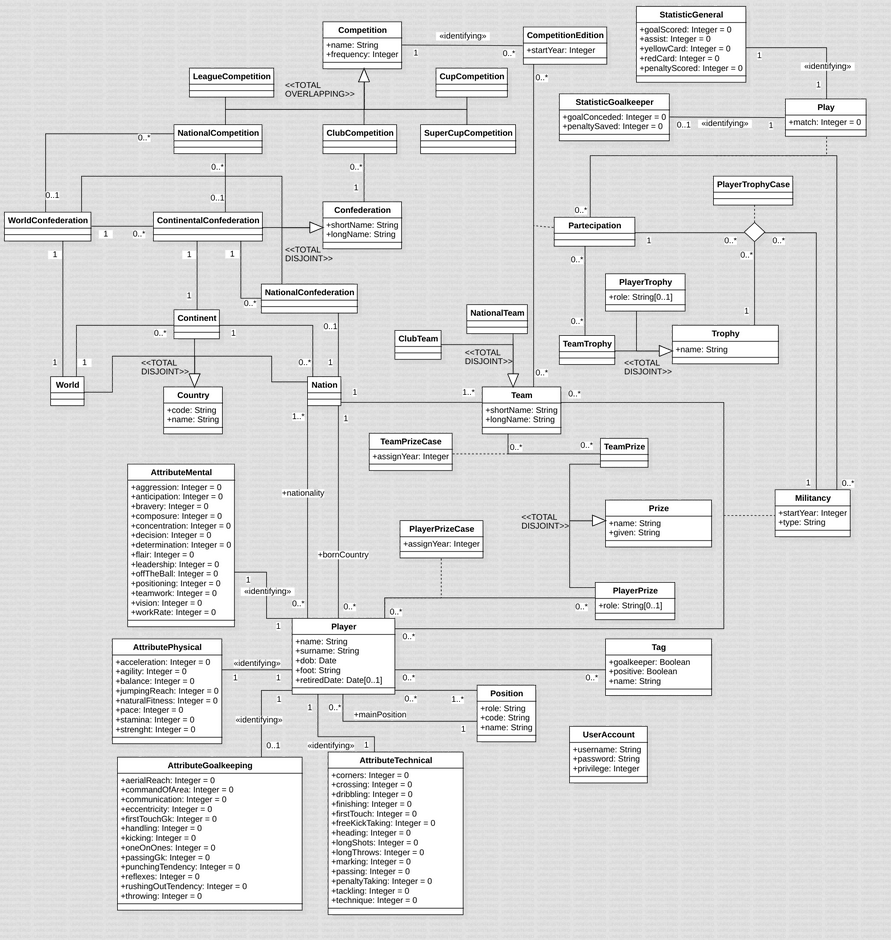
\includegraphics[width=\textwidth]{res/class_diagram_not_ristr}
\newpage

\subsubsection{\Large Ristrutturazione del Class Diagram}

\textbf{\large Analisi delle Ridondanze}

Possiamo constatare che non ci sono attributi ridondanti.

Notiamo però che vista l'alta frequenza di certe operazioni, 
che dovranno essere compiute sul database, vi è
un impellente necessità di introdurre delle ridondanze.


Un'operazione che deve essere effettuata ogni volta che
si voglia compiere una delle seguenti operazioni
per un calciatore:
\begin{itemize}
	\item Assegnare un trofeo;
	\item Aggiungere un valore di una statistica
		al play;
	\item Aggiungere un valore di un attributo;
	\item Assegnare un tag.
\end{itemize}
è quella di controllare quali sono i ruoli
che il calciatore ha giocato durante la sua carriera.
Questo ci porta quindi ad andare a controllare ogni volta
le sue posizioni di gioco ed estrarne i ruoli.

Per agevolare quest'operazione si è deciso di introdurre
una ridondanza nella classe Player, che appunto conservi
l'informazione sui ruoli in cui il calciatore fino a
quel momento ha giocato.
Per fare ciò si è deciso di creare un tipo enum
\textbf{enRoleMix} che contenga tutte le combinazioni
di ruoli possibili.



Un'altra operazione che si suppone sia ricorrente è
la visualizzazione delle 
nazionalità di un giocatore.

Questa informazione si potrebbe ottenere navigando 
entrambe le associazioni che \textbf{Player} ha con 
\textbf{Country}: bornCountry e Nationality.

Visto che quest'informazione è utile per un eventuale
controllo della militanza in nazionale e,
visto che il nostro database ha come scopo primario l'essere 
un sistema informativo per i calciatori, si vede necessario 
aggiungere alla relazione Nationality anche la nazione di 
nascita del calciatore così da velocizzare l'operazione, in 
quanto così facendo basta navigare soltanto l'associazione 
Nationality.


\newpage
\textbf{\large Eliminazione delle Generalizzazioni}

Nonostante le numerose generalizzazioni presenti nel Class 
Diagram, tutte hanno un qualcosa in comune, ovvero sono 
generalizzazioni disgiunte totali.

A seguito di ciò dunque, come metodo per eliminarle, si 
deciso di adottare l'accorpamento delle figlie della 
generalizzazione nel padre, aggiungendo dove necessario un 
attributo \textbf{type} che distinguesse le varie istanze 
della classe padre, e facendo le dovute correzioni ad 
eventuali attributi e/o associazioni delle classi figlie
con le altre classi.

Di seguito viene mostrato un elenco delle generalizzazioni e 
di come sono state ristrutturate:

\bigskip
\textbf{Country}
\bigskip

Alla classe \textbf{Country} è stato aggiunto un attributo 
\textbf{type} di tipo enum chiamato \textbf{enCountry}.
Il tipo \textbf{enCountry} può assumere tre valori:
\begin{itemize}
	\item Nation;
	\item Continental;
	\item World.
\end{itemize}

Per quanto riguarda le associazioni:

Le associazioni delle classi figlie di \textbf{Country} con 
le classi figlie di \textbf{Confederation} sono state 
accorpate, risultandone in un unica associazione tra 
\textbf{Country} e \textbf{Confederation} con molteplicità 
invariata.

Per quanto riguarda le associazioni della classe figlia 
\textbf{Nation} con \textbf{Player} e \textbf{Team}, esse 
sono state ricollegate alla classe padre \textbf{Country} 
mantenendo la molteplicità invariata.

\bigskip
\textbf{Confederation}
\bigskip

Alla classe \textbf{Confederation}  non è stato aggiunto un 
attributo \textbf{type} poiché si è sfruttato l'associazione 
1 a 1 (parziale) che le classi figlie di \textbf{Confederation}
avevano con le classi figlie di \textbf{Country}.
Dunque per comprendere a quale classe figlia una tupla di 
\textbf{Confederation} corrisponde, bisogna basarsi 
sull'attributo \textbf{type} della classe \textbf{Country}.

Per quanto riguarda le associazioni:

Le due associazioni che intercorrono tra le classi figlie di 
\textbf{Confederation}, ovvero l'associazione tra 
\textbf{NationalConfederation} e 
\textbf{ContinentalConfederation}, e tra 
\textbf{ContinentalConfederation} e 
\textbf{WorldConfederation}, sono state accorpate, 
risultandone in un'unica associazione tra la classe 
\textbf{Confederation} e sé stessa.

Le due associazioni delle classi figlie 
\textbf{ContinentalConfederation} e 
\textbf{WorldConfederation} con \textbf{NationalCompetition}, 
sono state accorpate, risultandone in un'unica associazione 
tra la classe \textbf{Confederation} e la classe 
\textbf{Competition}, classe padre di 
\textbf{NationalCompetition}.

L'associazione della classe figlia \textbf{NationalConfederation} e
\textbf{Team} è stata ricollegata alla classe padre mantenendo
molteplicità invariata.

\newpage
\textbf{Competition}
\bigskip

Alla classe \textbf{Competition} sono stati aggiunti due 
attributi: \textbf{type} di tipo enum chiamato 
\textbf{enCompetition} e \textbf{teamType} di tipo enum 
chiamato \textbf{enTeam}. Questo perché anche le classi 
figlie di \textbf{Competition} erano una generalizzazione a 
loro volta.

Nota che ci si è ridotti a solo due tipi aggiunti, perché le 
classi \textbf{NationalCompetition} e {ClubCompetition} hanno 
le stesse classi figlie.

Il tipo enum \textbf{enTeam} può assumere i seguenti valori:
\begin{itemize}
	\item National;
	\item Club.
\end{itemize}

Il tipo enum \textbf{enCompetition} può assumere i seguenti 
valori:
\begin{itemize}
	\item Cup;
	\item League;
	\item Super Cup.
\end{itemize}
Per quanto riguarda le associazioni:

L'associazione tra \textbf{ClubCompetition} e 
\textbf{Confederation}, è stata ricollegata alla classe padre 
\textbf{Competition} mantenendone però la molteplicità 
invariata.

\bigskip
\textbf{Team}
\bigskip

Alla classe \textbf{Team} è stato aggiunto un attributo 
\textbf{type} di tipo enum chiamato \textbf{enTeam} (lo 
stesso di Competition).

\bigskip
\textbf{Trophy}
\bigskip

Alla classe \textbf{Trophy} è stato aggiunto un attributo 
\textbf{type} di tipo enum chiamato \textbf{enAward} e l'attributo
\textbf{role} della classe figlia \textbf{PlayerTrophy}.

Il tipo \textbf{enAward} assume i seguenti valori:
\begin{itemize}
	\item Player
	\item Team
\end{itemize}
Per quanto riguarda le associazioni:

L'associazione tra \textbf{TeamTrophy} e 
\textbf{Partecipation} è stata ricollegata alla classe padre 
\textbf{Trophy} mantenendo la molteplicità invariata.


\bigskip
\textbf{Prize}
\bigskip

Alla classe \textbf{Prize} è stato aggiunto un attributo 
\textbf{type} di tipo enum chiamato \textbf{enAward} (lo 
stesso tipo di Trophy) e l'attributo
\textbf{role} della classe figlia \textbf{PlayerPrize}.

Per quanto riguarda le associazioni:

L'associazione tra \textbf{TeamPrize} e 
\textbf{Team} è stata ricollegata alla classe padre 
\textbf{Prize} mantenendo la molteplicità invariata.

L'associazione tra \textbf{PlayerPrize} e 
\textbf{Player} è stata ricollegata alla classe 
padre \textbf{Prize} mantenendo la molteplicità invariata.

\newpage
\textbf{\large Eliminazioni Attributi Multivalore}
\bigskip

Nel Class Diagram non sono presenti Attributi Multivalore.

\bigskip
\textbf{\large Eliminazione Attributi Strutturati}
\bigskip

Nel Class Diagram non sono presenti Attributi Strutturati.

\bigskip
\textbf{\large Partizionamento/Accorpamento di Entità
		e Associazioni}
\bigskip

L'unica accorpamento che potrebbe essere effettuato nel Class 
Diagram è quello tra \textbf{Country} e 
\textbf{Confederation}, poiché tra esse vi è un'associazione 
1 a 1 (parziale).

Si è arrivati però alla conclusione che c'è bisogno che le 
due classi siano separate, perché nelle altre associazioni 
che esse hanno con le altre classi, svolgono un ruolo 
centrale.

\newpage
\bigskip
\textbf{\large Scelta degli Identificatori Primari}
\bigskip

\newpage
\subsubsection{\Large Class Diagram ristrutturato}
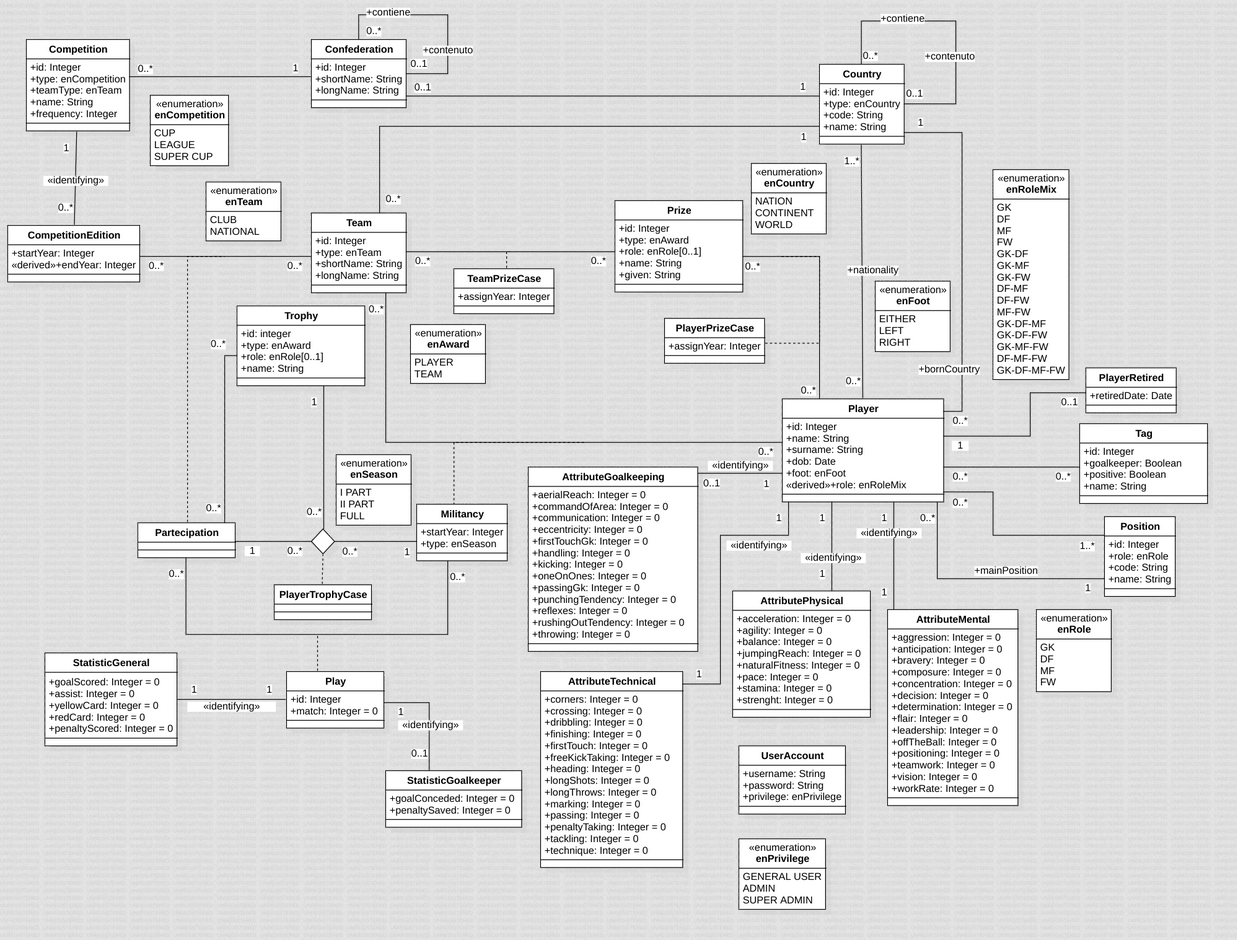
\includegraphics[width=\textwidth]{res/class_diagram_ristr}
\newpage

\subsubsection{\Large Dizionario}

\begin{center}
	\textbf{Dizionario delle Classi}
\end{center}


\begin{tblr}{
    hlines = {0.9pt}, vlines = {0.9pt}, colspec = {X[l]X[l]X[l]}, column{1}= {100pt},
    width = \textwidth, cell{1}{1-3} = {blue!10!white}
}
	{
		Classe
	}
	&
	{
		Descrizione
	}
	&
	{
		Attributo
	}
	\\
	{
		Attribute
	}
	&
	{
		Rappresenta gli attributi di un calciatore.
	}
	&
	{
		\textbf{id}(Integer)[chiave surrogata]:\\Rappresenta
			l'identificativo di un Attributo.\\
		\medskip\textbf{type}(enFeature):\\Rappresenta
			il tipo di un Attributo.\\
		\medskip\textbf{name}(String)[chiave naturale]:
			\\Rappresenta il nome di un Attributo.\\
		\medskip\textbf{description}(String)[parziale]:
			\\Rappresenta la descrizione di un Attributo.
	}
	\\
	{
		Competition
	}
	&
	{
		Rappresenta le competizioni calcistiche.
	}
	&
	{
		\textbf{id}(Integer)[chiave surrogata]:\\Rappresenta
			l'identificativo di una Competizione.\\
		\medskip\textbf{type}(enCompetition):\\Rappresenta
			il tipo di una Competizione.\\
		\medskip\textbf{teamType}(enTeam):\\Rappresenta
			il tipo di squadra che può
			partecipare alla Competizione.\\
		\medskip\textbf{name}(String)[chiave naturale]:
			\\Rappresenta il nome di una Competizione.\\
		\medskip\textbf{frequency}(Integer):\\Rappresenta
			la frequenza di una Competizione.
	}
	\\
	{
		CompetitionEdition
	}
	&
	{
		Rappresenta le edizioni delle competizioni calcistiche.
	}
	&
	{
		\textbf{startYear}(Integer)[chiave parziale]:
			\\Rappresenta l'anno di inizio di un'Edizione.\\
		\medskip\textbf{endYear}(Integer)[chiave parziale]:
			\\Rappresenta l'anno di fine di un'Edizione.\\
		\medskip\textbf{totalTeam}(Integer):\\Rappresenta
			il numero di team che partecipano in un'Edizione.
	}
	\\
	{
		Confederation
	}
	&
	{
	Rappresenta le confederazioni calcistiche.
	}
	& 
	{
		\textbf{id}(Integer)[chiave surrogata]:\\Rappresenta
			l'identificativo di una Confederazione.\\
		\medskip\textbf{shortName}(String):\\Rappresenta
			il nome abbreviato di una Confederazione.\\
		\medskip\textbf{longName}(String)[chiave naturale]:
			\\Rappresenta il nome esteso di una Confederazione.
	}
	\\
\end{tblr}

\newpage

\begin{tblr}{
    hlines = {0.9pt}, vlines = {0.9pt}, colspec = {X[l]X[l]X[l]}, column{1}= {100pt},
    width = \textwidth
}
	{
		Country
	}
	&
	{
		Rappresenta i paesi in cui si gioca
		ufficialmente a calcio.
	}
	&
	{
		\textbf{id}(Integer)[chiave surrogata]:\\Rappresenta
			l'identificativo di un Paese.\\
		\medskip\textbf{type}(enCountry):\\Rappresenta
			il tipo di un Paese.\\
		\medskip\textbf{code}(String)[chiave naturale]:
			\\Rappresenta il codice ISO 3166-1 alpha-3
			di un Paese.\\
		\medskip\textbf{name}(String)[chiave naturale]:
			\\Rappresenta il nome di un Paese.
	}
	\\
	{
		Player
	}
	&
	{
		Rappresenta i calciatori.
	}
	&
	{
		\textbf{id}(Integer)[chiave surrogata]:\\Rappresenta
			l'identificativo di un Calciatore.\\
		\medskip\textbf{name}(String):\\Rappresenta
			il nome di un Calciatore.\\
		\medskip\textbf{surname}(String):\\Rappresenta
			il cognome di un Calciatore.\\
		\medskip\textbf{dob}(Date):\\Rappresenta
			la data di nascita.\\
		\medskip\textbf{foot}(enFoot):\\Rappresenta
			il piede preferito di un Calciatore.\\
		\medskip\textbf{role}(enRoleMix)[derivato, parziale]:
			\\Rappresenta i possibili ruoli di gioco
			di un Calciatore.
	}
	\\
	{
		PlayerRetired
	}
	&
	{
		Rappresenta i calciatori che sono ritirati.
	}
	&
	{
		\textbf{retiredDate}(Date):\\Rappresenta
			la data di ritiro di un calciatore.
	}
	\\
	{
		Position
	}
	&
	{
		Rappresenta le posizioni di gioco di un Calciatore.
	}
	&
	{
		\textbf{id}(Integer)[chiave surrogata]:\\Rappresenta
			l'identificativo di una Posizione.\\
		\medskip\textbf{role}(enRole):\\Rappresenta
			il ruolo associato ad una Posizione.\\
		\medskip\textbf{code}(String)[chiave naturale]:
			\\Rappresenta il nome abbreviato di una Posizione.\\
		\medskip\textbf{name}(String)[chiave naturale]:
			\\Rappresenta il nome di una Posizione.
	}
	\\
\end{tblr}

\newpage

\begin{tblr}{
    hlines = {0.9pt}, vlines = {0.9pt}, colspec = {X[l]X[l]X[l]}, column{1}= {100pt},
    width = \textwidth
}

	{
		Prize
	}
	&
	{
		Rappresenta i premi calcistici.
	}
	&
	{
		\textbf{id}(Integer)[chiave surrogata]:\\Rappresenta
			l'identificativo del Premio.\\
		\medskip\textbf{type}(enAward):\\Rappresenta
			il tipo del Premio.\\
		\medskip\textbf{role}(enRole)[parziale]:\\Rappresenta
			il ruolo a cui è associato un Premio.\\
		\medskip\textbf{name}(String)[chiave naturale]:
			\\Rappresenta il nome del Premio.\\
		\medskip\textbf{description}(String)[parziale]:
			\\Rappresenta la descrizione del Premio.\\
		\medskip\textbf{given}(String):\\Rappresenta
			il nome della società calcistica
			che conferisce il Premio.
	}
	\\
	{
		Statistic
	}
	&
	{
		Rappresenta le statistiche di un calciatore.
	}
	&
	{
		\textbf{id}(Integer)[chiave surrogata]:\\Rappresenta
			l'identificativo della Statistica.\\
		\medskip\textbf{goalkeeper}(Boolean):\\Rappresenta
			se true che la Stastistica è associata
			soltanto al portiere, altrimenti a tutti i ruoli.\\
		\medskip\textbf{name}(String):\\Rappresenta
			il nome della Statistica.\\
		\medskip\textbf{description}(String)[parziale]:
			\\Rappresenta la descrizione della Statistica.
	}
	\\
	{
		Tag
	}
	&
	{
		Rappresenta i tag di un calciatore.
	}
	&
	{
		\textbf{id}(Integer)[chiave surrogata]:\\Rappresenta
			l'identificativo del Tag.\\
		\medskip\textbf{type}(enFeature):\\Rappresenta
			il tipo del Tag.\\
		\medskip\textbf{name}(String)[chiave naturale]:
			\\Rappresenta il nome del Tag.\\
		\medskip\textbf{description}(String)[parziale]:
			\\Rappresenta la descrizione del Tag.
	}
	\\
	{
		Team
	}
	&
	{
		Rappresenta le squadre di calcio.
	}
	&
	{
		\textbf{id}(Integer)[chiave surrogata]:\\Rappresenta
			l'identificativo della Squadra.\\
		\medskip\textbf{type}(enTeam):\\Rappresenta
			il tipo della Squadra.\\
		\medskip\textbf{name}(String)[chiave naturale]:
			\\Rappresenta il nome della Squadra.
	}
	\\
\end{tblr}

\newpage

\begin{tblr}{
    hlines = {0.9pt}, vlines = {0.9pt}, colspec = {X[l]X[l]X[l]}, column{1}= {100pt},
    width = \textwidth
}

	{
		Trophy
	}
	&
	{
		Rappresenta i trofei calcistici.
	}
	&
	{
		\textbf{id}(Integer)[chiave surrogata]:\\Rappresenta
			l'identificativo del Trofeo.\\
		\medskip\textbf{type}(enAward):\\Rappresenta
			il tipo del Trofeo.\\
		\medskip\textbf{role}(enRole)[parziale]:\\Rappresenta
			il ruolo a cui è associato un Trofeo.\\
		\medskip\textbf{name}(String)[chiave naturale]:
			\\Rappresenta il nome del Trofeo.\\
		\medskip\textbf{description}(String)[parziale]:
			\\Rappresenta la descrizione del Trofeo.\\
	}
	\\
	{
		UserAccount
	}
	&
	{
		Rappresenta gli utenti dell'applicativo.
	}
	&
	{
		\textbf{username}(String)[chiave naturale]:\\Rappresenta
			l'username dell'Account dell'Utente.\\
		\medskip\textbf{password}(String):\\Rappresenta
			la password dell'Account dell'Utente.\\
		\medskip\textbf{priviledge}(Integer):\\Rappresenta
			i privilegi dell'Account dell'Utente.
	}
	\\
\end{tblr}

\newpage

\begin{center}
	\textbf{Dizionario delle Associazioni}
\end{center}


\begin{tblr}{
    hlines = {0.9pt}, vlines = {0.9pt}, colspec = {X[l]X[l]X[l]X[l]}, column{1-2}= {100pt},
    width = \textwidth, cell{1}{1-4} = {blue!10!white}
}

	{
		Nome
	}
	&
	{
		Descrizione
	}
	&
	{
		Classe in Relazione
	}
	&
	{
		Attributo
	}
	\\
	{
		\textbf{Militancy}
	}
	&
	{
		Esprime le militanze di un calciatore in una squadra
		per stagione.
	}
	&
	{
		\textbf{Player [0 ... *]}:\\Indica che un Calciatore
			può militare in più Squadre.\\
		\medskip\textbf{Team [0 ... *]}:\\Indica che una Squadra
			può essere associata a più Calciatori.
	}
	&
	{
		\textbf{startYear}(Integer):\\Rappresenta
			la stagione di riferimento di una Militanza.\\
		\medskip\textbf{type}(enSeason):\\Rappresenta
			fino a che parte della stagione un Calciatore
			militava per quella Squadra.
	}
	\\
	{
		\textbf{PlayerPrizeCase}
	}
	&
	{
		Esprime i premi di un calciatore.
	}
	&
	{
		\textbf{Player [0 ... *]}:\\Indica che
			un Calciatore può essere associato a più Premi.\\
		\medskip\textbf{Prize [0 ... *]}:\\Indica che
			un Premio può essere associato, in anni diversi,
			a più Premi.
				
	}
	&
	{
		\textbf{assignYear}(Integer):\\Rappresenta
			l'anno di assegnazione del Premio al Calciatore.
	}
	\\
	{
		\textbf{Nationality}
	}
	&
	{
		Esprime le nazionalità di un calciatore.
	}
	&
	{
		\textbf{Country [0 ... *]}:\\Indica che
			uno stesso paese può essere associato a più
			calciatore.\\
		\medskip\textbf{Player [0 ... *]}:\\Indica che
			un calciatore può avere più nazionalità.
	}
	&
	{
	
	}
	\\
	{
		\textbf{bornCountry}
	}
	&
	{
		Esprime il paese di nascita di un calciatore.
	}
	&
	{
		\textbf{Country [0 ... *]}:\\Indica che
			un paese può essere il paese di nascita
			di più calciatori.\\
		\medskip\textbf{Player [1]}:\\Indica che
			un calciatore ha uno e un solo paese di nascita.
	}
	&
	{
	
	}
	\\
	{
		\textbf{Player-PlayerRetired}
	}
	&
	{
		Esprime i calciatori ritirati.
	}
	&
	{
		\textbf{Player [0 ... 1]}:\\Indica che
			un Calciatore può essere o non essere ritirato.\\
		\medskip\textbf{PlayerRetired [1]}:\\Indica che
			una data di ritiro si riferisce ad uno
			e un solo Calciatore. 
	}
	&
	{
	
	}
	\\
	{
		\textbf{Player-Tag}
	}
	&
	{
		Esprime i tag di un calciatore.
	}
	&
	{
		\textbf{Player [0 ... *]}:\\Indica che
			un Calciatore può essere associato a più Tag.\\
		\medskip\textbf{Tag [0 ... *]}:\\Indica che
			uno Tag può essere associato a più Calciatori.
	}
	&
	{
		
	}
	\\
\end{tblr}

\newpage

\begin{tblr}{
    hlines = {0.9pt}, vlines = {0.9pt}, colspec = {X[l]X[l]X[l]X[l]}, column{1-2}= {100pt},
    width = \textwidth
}

	{
		\textbf{Player-Position}
	}
	&
	{
		Esprime le posizioni di gioco di un calciatore.
	}
	&
	{
		\textbf{Player [0 ... *]}:\\Indica che
			un Calciatore può essere associato a più Posizioni.\\
		\medskip\textbf{Position [0 ... *]}:\\Indica che
			una Posizione può essere associata a più Calciatori.
	}
	&
	{
		
	}
	\\
	{
		\textbf{PlayerAttribute}
	}
	&
	{
		Esprime gli attributi di un calciatore.
	}
	&
	{
		\textbf{Player [0 ... *]}:\\Indica che un Calciatore
			può essere associato a più Attributi.\\
		\medskip\textbf{Attribute [0 ... *]}:\\Indica che 
			un Attributo può essere associato a più Calciatori.
	}
	&
	{
		\textbf{score}(Integer):\\Rappresenta il valore
			di un Attributo associato al Calciatore.
	}
	\\
	{
		\textbf{TeamPrizeCase}
	}
	&
	{
		Esprime i premi di una squadra.
	}
	&
	{
		\textbf{Team [0 ... *]}:\\Indica che
			una Squadra può essere associata a più Premi.\\
		\medskip\textbf{Prize [0 ... *]}:\\Indica che
			un Premio, in anni diversi, a più Squadre.
	}
	&
	{
		\textbf{assignYear}(Integer):\\Rappresenta
			l'anno di assegnazione di un Premio ad una Squadra.\\
	}
	\\
	{
		\textbf{Team-Country}
	}
	&
	{
		Esprime la nazionalità di una squadra.
	}
	&
	{
		\textbf{Team [1]}:\\Indica che una Squadra
			può essere associata ad un e un solo Paese.\\
		\medskip\textbf{Country [0 ... *]}:\\Indica che
			un Paese può essere associato a più Squadre.	
	}
	&
	{
		
	}
	\\
	{
		\textbf{Team-Confederation}
	}
	&
	{
		Esprime la confederazione di cui è membro una squadra.
	}
	&
	{
		\textbf{Team [1]}:\\Indica che una Squadra
			può essere associata ad un e un solo Paese.\\
		\medskip\textbf{Confederation [0 ... *]}:\\Indica che
			una Confederazione può essere associata
			a più Squadre.
	}
	&
	{
		
	}
	\\
	{
		\textbf{Partecipation}
	}
	&
	{
		Esprime  la partecipazione di una squadra
		ad un'edizione di una competizione.
	}
	&
	{
		\textbf{Team [0 ... *]}:\\Indica che una Squadra
			può partecipare a più Edizioni.\\
		\medskip\textbf{CompetitionEdition [0 ... *]}:
			\\Indica che una Edizione può essere associata
			a più squadre.

	}
	&
	{
		
	}
	\\
\end{tblr}

\newpage

\begin{tblr}{
    hlines = {0.9pt}, vlines = {0.9pt}, colspec = {X[l]X[l]X[l]X[l]}, column{1-2}= {100pt}, column{4}= {50pt},
    width = \textwidth
}

	{
		\textbf{Competition-CompetitionEdition}
	}
	&
	{
		Esprime le edizioni di una competizione.\\
		È una relazione identificante.
	}
	&
	{
		\textbf{Competition[0 ... *]}:\\Indica che
			una Competizione può essere associata
			a più Edizioni.\\
		\medskip\textbf{CompetitionEdition[1]}:\\Indica che
			un'Edizione può essere associata ad una
			e una sola Competizione.
	}
	&
	{
		
	}
	\\
	{
		\textbf{Competition-Confederation}
	}
	&
	{
		Esprime la confederazione che organizza
		la competizione.
	}
	&
	{
		\textbf{Competition [1]}:\\Indica che
			una Competizione può essere associata ad una
			e una sola Confederazione.\\
		\medskip\textbf{Confederation [0 ... *]}:\\Indica che
			una Confederazione può essere associata
			a più Competizioni.	
	}
	&
	{
		
	}
	\\
	{
		\textbf{Confederation-Confederation}
	}
	&
	{
		Esprime la possibilità di una confederazione di
		avere come membri altre confederazioni, o essere
		membro a sua volta.
	}
	&
	{
		\textbf{Confederation [0 ... 1] ruolo (contenuto)}:\\
			Indica che una Confederazione può o non può essere
			membra di un'altra Confederazione.\\
		\medskip\textbf{Confederation [0 ... *]
			ruolo (contiene)}:\\
			Indica che una Confederazione può essere associata
			a più Confederazioni.
	}
	&
	{
		
	}
	\\
	{
		\textbf{Confederation-Country}
	}
	&
	{
		Esprime l'appartenza di una confederazione
		ad un unico paese.
	}
	&
	{
		\textbf{Confederation [1]}:\\Indica che
			una Confederazione può essere associata
			ad un e un solo Paese.\\
		\medskip\textbf{Country [0 ... 1]}:\\Indica che
			un Paese può essere associata a nessuna o ad una
			Confederazione.
	}
	&
	{
		
	}
	\\
	{
		\textbf{Partecipation-Trophy}
	}
	&
	{
		Esprime la bacheca dei trofei di una squadra.
	}
	&
	{
		\textbf{Trophy [0 ... *]}:\\Indica che un Trofeo
			può essere associata a più Partecipazioni
			di una Squadra ad una Edizione.\\
		\medskip\textbf{Partecipation [0 ... *]}:\\Indica che
			una Partecipazione può essere associata
			a più Trofei.
	}
	&
	{
		
	}
	\\
	{
		\textbf{PlayerTrophyCase}	
	}
	&
	{
		Esprime la bacheca dei trofei di un calciatore.
	}
	&
	{
		\textbf{Partecipation [0 ... *]}:\\Indica che
			una Partecipazione può essere associata
			a più Bacheche.\\
		\medskip\textbf{Trophy [0 ... *]}:\\Indica che
			un Trofeo può essere associato
			a più Bacheche.\\
		\medskip\textbf{Militancy [0 ... *]}:\\Indica che
			una Militanza può essere associata
			a più Bacheche.\\
		\medskip\textbf{PlayTrophyCase -> Partecipation [1]}:
			\\Indica che una Bacheca può essere associata
			ad una e una sola Partecipazione.\\
		\medskip\textbf{PlayTrophyCase -> Trophy [1]}:
			\\Indica che una Bacheca può essere associata
			ad un e un solo Trofeo.\\
		\medskip\textbf{PlayTrophyCase -> Militancy [1]}:
			\\Indica che una Bacheca può essere associata
			ad una e una sola Militanza.
	}
	&
	{
		
	}
	\\
\end{tblr}

\newpage

\begin{tblr}{
    hlines = {0.9pt}, vlines = {0.9pt}, colspec = {X[l]X[l]X[l]X[l]}, column{1-2}= {100pt},
    width = \textwidth
}

	{
		\textbf{Play}
	}
	&
	{
		Esprime in quale edizione di una competizione
		un calciatore, che militava per una certa squadra,
		ha giocato.
	}
	&
	{
		\textbf{Partecipation [0 ... *]}:\\Indica che
			una Partecipazione può essere associata
			a più Rose.\\
		\medskip\textbf{Militancy [0 ... *]}:\\Indica che
			una Militanza può essere associata
			a più Partecipazioni.
	}
	&
	{
		\textbf{id}(Integer)[chiave surrogata]:\\Rappresenta
			l'identificativo di un Gioco.\\
		\medskip\textbf{match}(Integer):\\Rappresenta
			il numero di presenze di un calciatore
			in un Gioco.
	}
	\\
	{
		\textbf{PlayStatistic}
	}
	&
	{
		Esprime le statistiche di un gioco.
	}
	&
	{
		\textbf{Play [0 ... *]}:\\Indica che
			un Gioco può essere associato
			a più Statistiche.\\
		\medskip\textbf{Statistic [0 ... *]}:\\Indica che
			una Statistica può essere associata
			a più Giochi.\\
	}
	&
	{
		\textbf{score}(Integer):\\Rappresenta
			il valore di una Statistica per un Gioco.
	}
	\\
\end{tblr}


\newpage

\begin{center}
	\textbf{Dizionario dei Vincoli}
\end{center}

\begin{tblr}{
    hlines = {0.9pt}, vlines = {0.9pt}, colspec = {X[l]X[l]X[l]}, 
    width = \textwidth, cell{1}{1-3} = {blue!10!white}
}
	{
		Vincolo
	}
	&
	{
		Tipo
	}
	&
	{
		Descrizione
	}
	\\
	{
		uqCountryCode
	}
	&
	{
		INTRARELAZIONALI
	}
	&
	{
		Non possono esistere paesi diversi con
		lo stesso codice.
	}
	\\
	{
		uqCountryName
	}
	&
	{
		INTRARELAZIONALI
	}
	&
	{
		Non possono esistere paesi diversi con
		lo stesso nome.
	}
	\\
	{
		uqConfederationLongName
	}
	&
	{
		INTRARELAZIONALI
	}
	&
	{
		Non possono esistere confederazioni calcistiche
		diverse con lo stesso nome esteso.
	}
	\\
	{
		Controllo ConfederationSuper
	}
	&
	{
		INTRARELAZIONALI
	}
	&
	{
		Una confederazione deve essere membro soltanto di una
		una confederazione con tipo strettamente superiore.
	}
	\\
	{
		uqTeam
	}
	&
	{
		INTRARELAZIONALI
	}
	&
	{
		Non possono esistere squadre di calcio diverse
		con lo stesso nome.
	}
	\\
	{
		Controllo TeamCountry
	}
	&
	{
		INTERELAZIONALI
	}
	&
	{
		Una squadra di calcio deve essere associata soltanto
		ad un paese che sia una nazione.
		
	}
	\\
	{
		Controllo TeamConf
	}
	&
	{
		INTERELAZIONALI
	}
	&
	{
		Una squadra di calcio deve essere associata soltanto
		alla confederazione che abbia come paese associato
		lo stesso della squadra.
	}
	\\
	{
		Controllo TeamNatName
	}
	&
	{
		INTERELAZIONALI
	}
	&
	{
		Una squadra di calcio nazionale deve avere come nome
		lo stesso del paese associato.
	}
	\\
	{
		uqCompetitionName
	}
	&
	{
		INTRARELAZIONALI
	}
	&
	{
		Non possono esistere competizioni calcistiche
		diverse con lo stesso nome.
	}
	\\
	{
		Controllo Comp
	}
	&
	{
		INTERELAZIONALI
	}
	&
	{
		Una competizione calcistica tra squadre nazionali
		non deve avere associata una confederazione
		di tipo nazionale.
	}
	\\
	{
		uqCompetitionEditionEndYear
	}
	&
	{
		INTRARELAZIONALI
	}
	&
	{
		Ogni edizione di una competizione calcistica
		deve finire in un anno diverso.
	}
	\\
	{
		ckCompetitionEditionRange
	}
	&
	{
		N-UPLA
	}
	&
	{
		Ogni edizione di una competizione calcistica deve
		iniziare e finire nello stesso anno o
		al massimo terminare l'anno successivo
		a quello di inizio.
	}
	\\
	{
		ckCompetitionEditionTotalTeam
	}
	&
	{
		N-UPLA
	}
	&
	{
		Il numero di squadre di calcio che possono partecipare
		ad una edizione di una competizione calcistica
		deve essere compreso tra un minimo di 2 ed
		un massimo di 128.
	}
	\\
	{
		Controllo CompEdLeagueYears
	}
	&
	{
		INTERELAZIONALI
	}
	&
	{
		Un'edizione di una competizione calcistica
		di tipo campionato non deve iniziare
		e finire nello stesso anno.
	}
	\\
\end{tblr}

\newpage

\begin{tblr}{
    hlines = {0.9pt}, vlines = {0.9pt}, colspec = {X[l]X[l]X[l]}, 
    width = \textwidth
}

	{
		Controllo CompEdSuperCupYears
	}
	&
	{
		INTERELAZIONALI
	}
	&
	{
		Un'edizione di una competizione calcistica
		di tipo supercoppa deve iniziare
		e finire nello stesso anno.
	}
	\\
	{
		Controllo CompEdCupNatYears
	}
	&
	{
		INTERELAZIONALI
	}
	&
	{
		Un'edizione di una competizione calcistica
		di tipo coppa tra squadre nazionali deve
		iniziare e finire nello stesso anno.
	}
	\\
	{
		Controllo CompEdCupClubYears
	}
	&
	{
		INTERELAZIONALI
	}
	&
	{
		Un'edizione di una competizione calcistica
		di tipo coppa tra squadre club non deve
		iniziare e finire nello stesso anno.
	}
	\\
	{
		Controllo CompEdSuperCupTotTeam
	}
	&
	{
		INTERELAZIONALI
	}
	&
	{
		Un'edizione di una competizione calcistica
		di tipo SuperCoppa deve avere al massimo
		sei squadre di calcio partecipanti.
	}
	\\
	{
		Controllo CompEdLeagueTotTeam
	}
	&
	{
		INTERELAZIONALI
	}
	&
	{
		Un'edizione di una competizione calcistica
		di tipo campionato deve avere al massimo
		cinquanta squadre di calcio partecipanti.
	}
	\\
	{
		Controllo CompEdCupNatTotTeam
	}
	&
	{
		INTERELAZIONALI
	}
	&
	{
		Un'edizione di una competizione calcistica
		di tipo coppa, organizzata da una confederazione
		di tipo nazionale, deve avere come numero
		di squadre di calcio partecipanti una potenza di due
	}
	\\
	{
		Controllo CompEdCupIntTotTeam
	}
	&
	{
		INTERELAZIONALI
	}
	&
	{
		Un'edizione di una competizione calcistica
		di tipo coppa, organizzata da una confederazione
		di tipo diverso da nazionale, deve avere al massimo
		cinquanta squadre di calcio partecipanti.	
	}
	\\
	{
		Controllo CompEdFreq
	}
	&
	{
		INTERELAZIONALI
	}
	&
	{
		L'anno di inizio e fine di un'edizione
		di una competizione calcistica, deve rispettare
		la frequenza della sua competizione di riferimento.
		
	}
	\\
	{
		Controllo PartTotTeam
	}
	&
	{
		INTERELAZIONALI
	}
	&
	{
		La partecipazione di una squadra di calcio
		ad un'edizione di una competizione calcistica
		deve essere accettata soltanto se
		il numero massimo di squadre partecipanti per
		quell'edizione non è stato superato.
	}
	\\
	{
		Controllo PartTeamConf
	}
	&
	{
		INTERELAZIONALI
	}
	&
	{
		La partecipazione di una squadra di calcio
		ad un'edizione di una competizione calcistica
		deve essere accettata soltanto se
		la confederazione che organizza
		la competizione calcistica, è la stessa
		della squadra di calcio oppure contiene
		la confederazione associata alla squadra di calcio.
	}
	\\
\end{tblr}


\newpage

\begin{tblr}{
    hlines = {0.9pt}, vlines = {0.9pt}, colspec = {X[l]X[l]X[l]}, 
    width = \textwidth
}

	{
		Controllo PartTeamType
	}
	&
	{
		INTERELAZIONALI
	}
	&
	{
		La partecipazione di una squadra di calcio
		ad un'edizione di una competizione calcistica
		deve essere accettata soltanto se
		il tipo di squadra della competizione calcistica
		è lo stesso della squadra di calcio
		in considerazione.
	}
	\\
	{
		Controllo PartTeamComp
	}
	&
	{
		INTERELAZIONALI
	}
	&
	{
		La partecipazione di una squadra di calcio
		ad un'edizione di una competizione calcistica
		deve essere accettata soltanto se
		la squadra non partecipi già ad un'altra edizione
		di una competizione calcistica dello stesso tipo,
		nello stesso anno e organizzata dalla
		stessa confederazione.
	}
	\\
	{
		uqPlayer
	}
	&
	{
		INTRARELAZIONALI	
	}
	&
	{
		Non possono esistere calciatori diversi
		con la stessa combinazione di nome,
		cognome, data di nascita e paese di nascita.
	}
	\\
	{
		Controllo PlayerNat
	}
	&
	{
		INTERELAZIONALI
	}
	&
	{
		Un calciatore deve essere
		associato ad un paese che sia una nazione.
	}
	\\
	{
		Controllo PlayerRole
	}
	&
	{
		N-UPLA
	}
	&
	{
		Un calciatore, nel momento dell'inserimento,
		deve avere come valore dell'attributo role
		NULL.
	}
	\\
	{
		Controllo PlayerRetired
	}
	&
	{
		INTERELAZIONALI
	}
	&
	{
		La data di ritiro di un calciatore deve
		essere successiva alla data di nascita più
		un minimo età per diventare un calciatore,
		più di sei mesi di attività professionale.
	}
	\\
	{
		Controllo PlayerRetiredMilitancy
	}
	&
	{
		INTERELAZIONALI
	}
	&
	{
		La data di ritiro di un calciatore deve
		essere uguale o successiva all'anno
		dell'ultima, in ordine di anni crescente,
		militanza del calciatore.
	}
	\\
	{
		ckMilitancy
	}
	&
	{
		N-UPLA
	}
	&
	{
		 La militanza per un calciatore in una squadra nazionale
		 deve durare per l'intera stagione in cui è stato convocato.
	}
	\\
	{
		Controllo MilitancyPlayer
	}
	&
	{
		INTERELAZIONALI
	}
	&
	{
		Una militanza di un	calciatore per
		una squadra di calcio deve essere accettata
		soltanto se il calciatore ha almeno
		una posizione di gioco.
	}
	\\
	{
		Controllo MilitancyValidRange
	}
	&
	{
		INTERELAZIONALI
	}
	&
	{
		L'anno della militanza di un calciatore
		per una squadra di calcio deve essere
		un anno valido per il calciatore.
	}
	\\
	{
		Controllo MilitancyTeamNatPlayer
	}
	&
	{
		INTERELAZIONALI	
	}
	&
	{
		La militanza di un calciatore per
		una squadra di calcio nazionale deve
		essere accettata se il paese associato
		alla squadra di calcio nazionale è una
		nazionalità del calciatore.
	}
	\\
\end{tblr}

\newpage


\begin{tblr}{
    hlines = {0.9pt}, vlines = {0.9pt}, colspec = {X[l]X[l]X[l]}, 
    width = \textwidth
}
	{
		Controllo MilitancyTeamNat
	}
	&
	{
		INTRARELAZIONALI
	}
	&
	{
		La militanza di un calciatore per
		una squadra di calcio nazionale deve
		essere accettata se il calciatore non ha
		nessuna militanza con altre
		squadre di calcio nazionali.
	}
	\\
	{
		Controllo Militancy
	}
	&
	{
		INTRARELAZIONALI	
	}
	&
	{
		La militanza di un calciatore per
		una squadra di calcio deve essere
		accettata se non vi è una sovrapposizione
		temporale con altre militanze dello
		stesso calciatore per altre squadre di calcio
		dello stesso tipo di quella in considerazione.
	}
	\\
	{
		uqTagName
	}
	&
	{
		INTRARELAZIONALI
	}
	&
	{
		Non possono esistere tag diversi con
		lo stesso nome.
	}
	\\
	{
		uqTagDescription
	}
	&
	{
		INTRARELAZIONALI
	}
	&
	{
		Non possono esistere tag diversi con
		la stessa descrizione.
	}
	\\
	{
		Controllo PlayerTagGK
	}
	&
	{
		INTERELAZIONALI
	}
	&
	{
		Un Tag di tipo portiere deve essere associato
		ad un calciatore soltanto se portiere è uno dei
		ruoli in campo del calciatore.
	}
	\\
	{
		uqPositionCode
	}
	&
	{
		INTRARELAZIONALI
	}
	&
	{
		Non possono esistere posizioni di gioco
		diverse con lo stesso codice.
	}
	\\
	{
		uqPositionName
	}
	&
	{
		INTRARELAZIONALI
	}
	&
	{
		Non possono esistere posizioni di gioco
		diverse con lo stesso nome.
	}
	\\
	{
		uqAttributeName
	}
	&
	{
		INTRARELAZIONALI
	}
	&
	{
		Non possono esistere attributi diversi
		con lo stesso nome.
	}
	\\
	{
		uqAttributeDescription
	}
	&
	{
		INTRARELAZIONALI
	}
	&
	{
		Non possono esistere attributi diversi
		con la stessa descrizione.
	}
	\\
	{
		Controllo PlayerAttributeGK
	}
	&
	{
		INTERELAZIONALI
	}
	&
	{
		Un Attributo di tipo portiere deve essere associato
		ad un calciatore soltanto se portiere è uno dei
		ruoli in campo del calciatore.
	}
	\\
	{
		uqStatisticName
	}
	&
	{
		INTRARELAZIONALI
	}
	&
	{
		Non possono esistere statistiche diverse
		con lo stesso nome.
	}
	\\
	{
		uqStatisticDescription
	}
	&
	{
		INTRARELAZIONALI
	}
	&
	{
		Non possono esistere statistiche diverse
		con la stessa descrizone.
	}
	\\
	{
		uqTrophyName
	}
	&
	{
		INTRARELAZIONALI
	}
	&
	{
		 Non possono esistere trofei calcistici diversi
		 con lo stesso nome.
	}
	\\
	{
		uqTrophyDescription
	}
	&
	{
		INTRARELAZIONALI
	}
	&
	{
		Non possono esistere trofei calcistici diversi
		con la stessa descrizione.
	}
	\\
	{
		ckTrophy
	}
	&
	{
		N-UPLA
	}
	&
	{
		I trofei di squadra non devono essere associati
		ad alcun ruolo.
	}
	\\
	{
		Controllo TeamTrophyCase
	}
	&
	{
		INTERELAZIONALI
	}
	&
	{
		Una squadra di calcio deve essere associata
		soltanto a trofei di tipo squadra.
	}
	\\
\end{tblr}

\newpage

\begin{tblr}{
    hlines = {0.9pt}, vlines = {0.9pt}, colspec = {X[l]X[l]X[l]}, 
    width = \textwidth
}

	{
		Controllo PlayerTrophyCaseMil
	}
	&
	{
		INTERELAZIONALI
	}
	&
	{
		Un trofeo deve essere associato ad 
		un calciatore soltanto se la sua militanza,
		nella stagione in cui è stato vinto il trofeo,
		non è stata per la prima parte.
	}
	\\
	{
		Controllo PlayerTrophyCaseTeam
	}
	&
	{
		INTERELAZIONALI
	}
	&
	{
		Un trofeo di tipo squadra deve essere associato
		ad un calciatore soltanto se la squadra di calcio
		in cui il calciatore militava nella stagione
		di assegnazione del trofeo, ha vinto quel trofeo.
	}
	\\
	{
		Controllo PlayerTrophyCaseRole
	}
	&
	{
		INTERELAZIONALI
	}
	&
	{
		Un trofeo di tipo calciatore
		in uno specifico ruolo deve essere associato
		ad un calciatore soltanto se il ruolo a cui
		è associato il trofeo è un ruolo di gioco
		del calciatore
	}
	\\
	{
		uqPrizeName
	}
	&
	{
		INTRARELAZIONALI
	}
	&
	{
		Non possono esistere premi calcistici diversi
		con lo stesso nome.
	}
	\\
	{
		uqPrizeDescription
	}
	&
	{
		INTRARELAZIONALI
	}
	&
	{
		Non possono esistere premi calcistici diversi
		con la stessa descrizione.
	}
	\\
	{
		ckPrize
	}
	&
	{
		N-UPLA
	}
	&
	{
		I premi di squadra non devono essere associati
		ad alcun ruolo.
	}
	\\
	{
		Controllo TeamPrize
	}
	&
	{
		INTERELAZIONALI
	}
	&
	{
		Una squadra di calcio deve essere associata
		soltanto a premi di tipo squadra.
	}
	\\
	{
		Controllo PlayerPrize
	}
	&
	{
		INTERELAZIONALI
	}
	&
	{
		Un calciatore deve essere associato soltanto
		a premi di tipo calciatore.
	}
	\\
	{
		Controllo PlayerPrizeValidRange
	}
	&
	{
		INTERELAZIONALI	
	}
	&
	{
		L'anno di assegnazione di un premio ad
		un calciatore deve essere un anno valido
		del calciatore.
	}
	\\
	{
		Controllo PlayerPrizeRole
	}
	&
	{
		INTERELAZIONALI
	}
	&
	{
		Un premio di tipo calciatore
		in uno specifico ruolo deve essere associato
		ad un calciatore soltanto se il ruolo a cui
		è associato il premio è un ruolo di gioco
		del calciatore.
	}
	\\
	{
		uqPlay
	}
	&
	{
		INTRARELAZIONALI
	}
	&
	{
		TODO
	}
	\\
	{
		ckPlay
	}
	&
	{
		N-UPLA
	}
	&
	{
		Il numero di presenze di un calciatore in un gioco
		deve essere maggiore di zero.
	}
	\\
	{
		Controllo PlayMatch
	}
	&
	{
		INTERELAZIONALI
	}
	&
	{
		Il numero di match di un gioco deve essere
		al massimo pari al numero di squadre, che
		possono partecipare all'edizione della competizione
		associata, moltiplicato per quattro.
	}
	\\
	{
		Controllo StatisticRole
	}
	&
	{
		INTERELAZIONALI
	}
	&
	{
		Una statistica che abbia l'attributo goalkeeper
		true deve essere associata ad un gioco
		soltanto se il calciatore associato ha tra
		i suoi ruoli di gioco il portiere.
	}
	\\
\end{tblr}


\newpage

\begin{tblr}{
    hlines = {0.9pt}, vlines = {0.9pt}, colspec = {X[l]X[l]X[l]},  column{1-2}={100pt},
    width = \textwidth
}
	
	{
		dmAlnum
	}
	&
	{
		DOMINIO
	}
	&
	{
		Dominio per gli attributi delle seguenti classi:\\
		shortName e longName di Confederation;\\
		name di Team;\\
		name di Competition.\\
		Questo dominio sfrutta le espressioni regolari
		per accettare soltanto strighe alfanumeriche
		(comprese lettere accentate) che abbiano
		una lunghezza compresa tra due e cento caratteri,
		ed evitare eventuali ripetizioni di caratteri
		di punteggiatura e spazi non validi.
	}
	\\
	{
		dmDate
	}
	&
	{
		DOMINIO
	}
	&
	{
		Dominio per tutti gli attributi di tipo Date.
		Questo dominio non permette l'inserimento di
		date che siano successive alla data corrente.
	}
	\\
	{
		dmString
	}
	&
	{
		DOMINIO
	}
	&
	{
		Dominio per tutti i restanti attributi di tipo
		String tranne l' attributo descrizione
		eventualmente presente nella classe.
		Questo dominio sfrutta le espressioni
		regolari per accettare soltanto stringhe
		(comprese lettere accentate) che abbiano
		una lunghezza compresa tra due e cento caratteri.
		Questo dominio inoltre blocca l'inserimento
		di strighe con ripetizioni di segni
		di punteggiatura e spazi che non siano validi.
	}
	\\
	{
		dmPassword
	}
	&
	{
		DOMINIO
	}
	&
	{
		Dominio per l'attributo password di UserAccount.
		Questo dominio sfrutta le espressioni regolari
		per controllare che siano stati inseriti
		un numero, una lettera minuscola e maiuscola
		e un carattere speciale e che la sua lunghezza
		sia compresa tra otto e duecentocinquantacinque
		caratteri.
	}
	\\
	{
		dmUsername
	}
	&
	{
		DOMINIO
	}
	&
	{
		Dominio per l'attributo username di UserAccount.
		Questo dominio sfrutta le espressioni regolari
		per accettare una stringa di
		caratteri alfanumerici, punti,
		trattini e underscore,
		con una lunghezza compresa tra due e diciotto
		caratteri. Questo dominio inoltre blocca
		ripetizioni e composizioni di segni
		di punteggiatura non validi.
		
	}
	\\
	{
		dmCode
	}
	&
	{
		DOMINIO
	}
	&
	{
		Dominio per gli attributi code delle classi:
		country e position.
		Questo dominio sfrutta le espressioni regolari
		per accettare stringhe dell'alfabeto maiuscole
		che abbiano una lunghezza compresa tra
		due e tre caratteri.
	}
	\\
	{
		dmYear
	}
	&
	{
		DOMINIO
	}
	&
	{
		Dominio per gli attributi year delle classi:
		CompetitionEdition, TeamPrizeCase e
		PlayerPrizeCase.
		Questo dominio non permette di far inserire
		anni strettamente successivi
		all'anno corrente più uno.
	}
	\\
	{
		dmUint
	}
	&
	{
		DOMINIO
	}
	&
	{
		Dominio per tutti i restanti attributi
		di tipo integer.
		Questo dominio non permette di far inserire
		valori numerici inferiori allo zero.
	}
	\\
\end{tblr}

